\documentclass[10pt,a4paper]{article}
\usepackage[utf8]{inputenc}
\usepackage{amsmath}
\usepackage{amsfonts}
\usepackage{amssymb}
\usepackage{tikz}
\usetikzlibrary{angles}
\usetikzlibrary{quotes}
\begin{document}
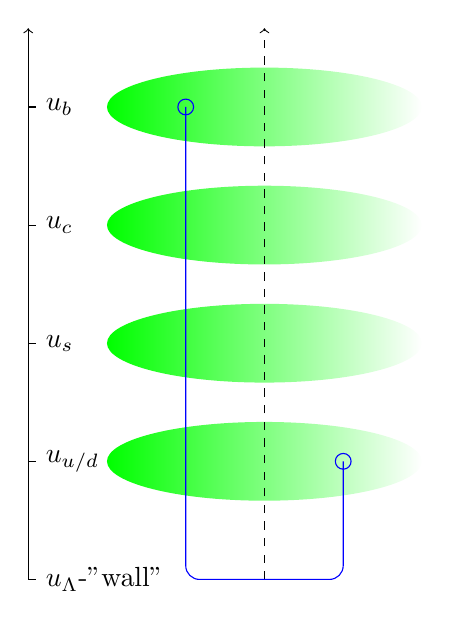
\begin{tikzpicture}[rounded corners=5pt,scale=0.1]
\shade[left color=green,right color=white] (30,15) ellipse [x radius=20,y radius=5];
\shade[left color=green,right color=white] (30,30) ellipse [x radius=20,y radius=5];
\shade[left color=green,right color=white] (30,45) ellipse [x radius=20,y radius=5];
\shade[left color=green,right color=white] (30,60) ellipse [x radius=20,y radius=5];
\draw[dashed,->] (30,0) -- (30,70);
\draw[->] (0,0) -- (0,70);
\draw[color=blue] (20,60) circle [radius=1,fill=blue]--(20,0)--(40,0)--(40,15) circle [radius=1,fill=blue];
\draw (0,0)--(1,0) node[anchor=west] {$u_\Lambda$-"wall"};
\draw (0,15)--(1,15) node[anchor=west] {$u_{u/d}$};
\draw (0,30)--(1,30) node[anchor=west] {$u_s$};
\draw (0,45)--(1,45) node[anchor=west] {$u_c$};
\draw (0,60)--(1,60) node[anchor=west] {$u_b$};
\end{tikzpicture}
\end{document}